%!TEX root = ../dokumentation.tex

\section{Architektur der Anwendung}
Im folgenden Abschnitt soll die Architektur der Implementierung erläutert werden. Des Weiteren wird beleuchtet, wie die Datenmodellierung in \acs{Redis} realisiert wurde.

Wie bereits im vorangegangen Abschnitt erwähnt, soll eine Chat-App implementiert werden. Die Anwendung besteht aus zwei Hauptkomponenten: dem Backend und dem Frontend (vgl. \autoref{fig:arch}). Die Aufgabe des Frontend ist es, dem Benutzer eine \acs{GUI} zu präsentieren. Alle Eingaben des Benutzers werden im Backend ausgewertet. Zwischen beiden Komponenten besteht eine bidirektionale Kommunikation. Das Frontend sendet den Input des Benutzers und das Backend sendet nötige Änderungen.
\begin{figure}[h]
	\centering
	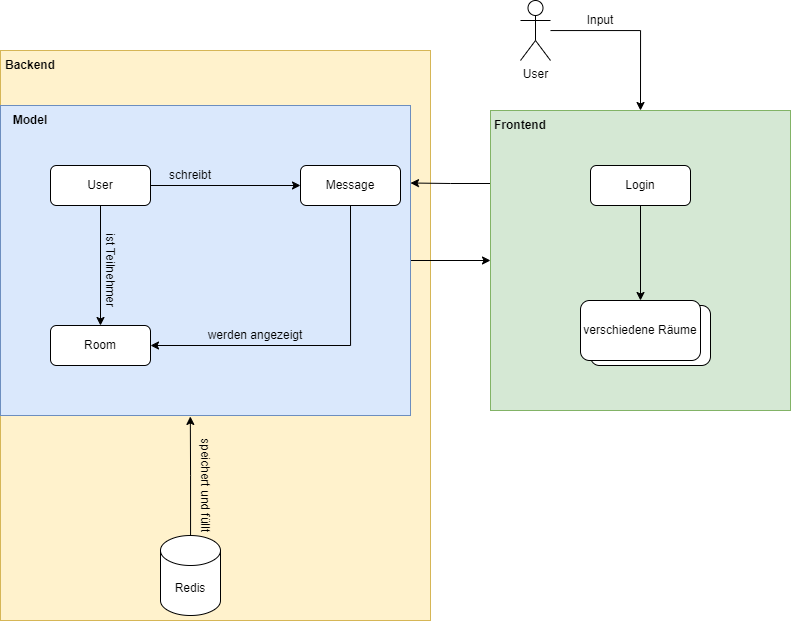
\includegraphics[width=0.7\textwidth]{redis_arch.png}
	\caption{Architektur der Chat-App}
	\label{fig:arch}
\end{figure}

Das Backend besteht aus zwei Teilen. Zum einen aus dem Model der Applikation, zum Anderen aus einer \acs{Redis}-Datenbank (vgl. \autoref{fig:arch}). Das Model ist ein objekt- orientierter Ansatz zur Modellierung der benötigten Daten. Es besteht aus einer \textit{User} Klasse, welche alle Informationen, wie Name, E-Mail und Passwort eines User speichert, einer \textit{Message} Klasse, welche Nachrichten repräsentiert, die ein User in einen bestimmten Raum sendet und einer \textit{Room} Klasse, welche einen spezifischen Chatraum darstellt. Jedes \textit{Room} Objekt hat zwei Teilnehmer und eine Menge an Nachrichten. Der objektorientierte Ansatz wurde gewählt, um die Daten mithilfe eines \acs{ORM} Ansatzes aus der Datenbank in die Applikation zu integrieren. Auf diese Weise kann den Daten eine semantische Bedeutung gegeben werden und die Weiterverarbeitung wird erleichtert.

In der \acs{Redis}-Datenbank werden verschiedene Datentypen verwendet, um deren Unterschiede zu demonstrieren. Die verwendeten Datentypen sind Hashes und Sorted Sets (vgl. \autoref{subsec:datentypen}). Für die Speicherung der User-Daten wurden Hashes verwendet. Mit dieser Herangehensweise kann jeder User anhand eines Schlüssels identifiziert werden (vgl. \autoref{fig:sub1}).

Die Räume wurden mithilfe von Sorted-Sets realisiert. Ein Raum besteht aus zwei Teilnehmern und einer Menge an Nachrichten. Die Teilnehmer werden mittels den festen Scores \textit{-2} und \textit{-1} identifiziert. Bei Abfrage dieser Score liefert die Datenbank den Schlüssel des zugehörigen Users. Alle weiteren Scores sind die Timestamps der zugehörigen Nachricht, welche in einem \acs{JSON} ähnlichen Format abgespeichert wird (vgl. Abbildung \ref{fig:sub3}).

In \acs{Redis} ist es möglich Bilder in Form einer Bitmap zu speichern. Die Avatare (= Profilbilder der User) werden ebenfalls in Sorted Sets gespeichert. Diese sind als Bitmap abgelegt und können anhand ihres Scores abgefragt und in der Applikation zurück in ein Bild umgewandelt werden (vgl. Abbildung \ref{fig:sub3}).
\begin{figure}[h]
	\centering
	
	\begin{subfigure}{0.3\textwidth}
		\centering
		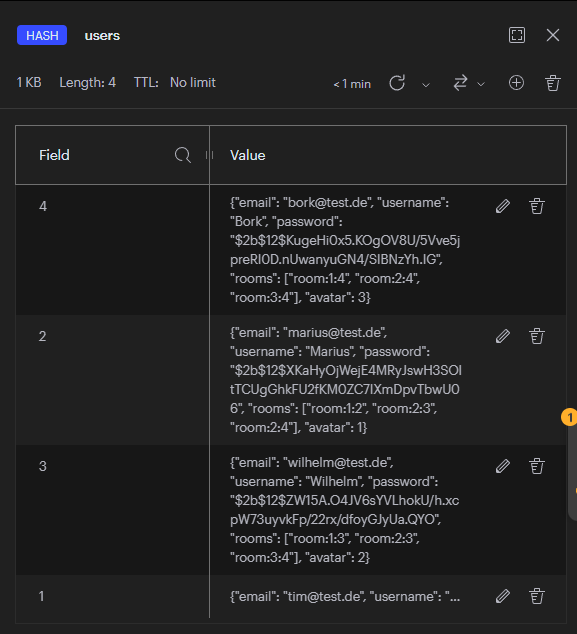
\includegraphics[width=\linewidth]{user_hash.png}
		\caption{Speicherung der User}
		\label{fig:sub1}
	\end{subfigure}%
	\hspace{0.02\textwidth}
	\begin{subfigure}{0.3\textwidth}
		\centering
		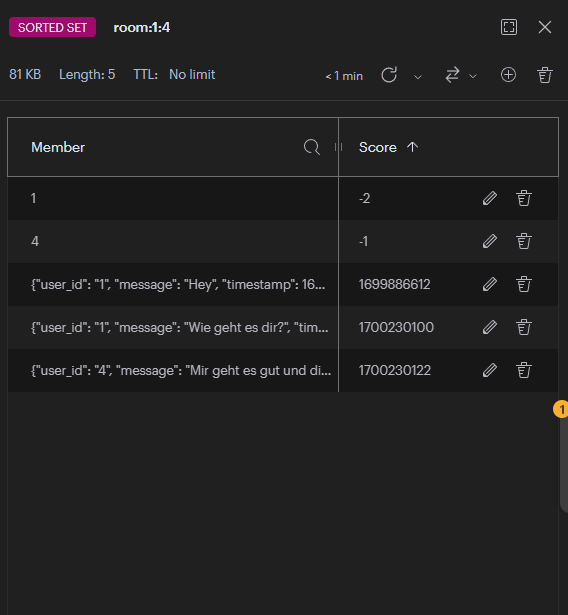
\includegraphics[width=\linewidth]{room.png}
		\caption{Speicherung der Räume}
		\label{fig:sub2}
	\end{subfigure}%
	\hspace{0.02\textwidth}
	\begin{subfigure}{0.3\textwidth}
		\centering
		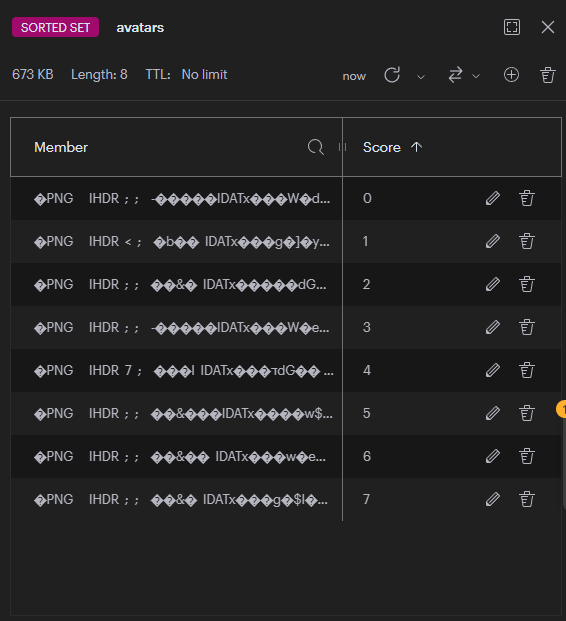
\includegraphics[width=\linewidth]{avatars.png}
		\caption{Speicherung der Avatare}
		\label{fig:sub3}
	\end{subfigure}
	
	\caption{Datenmodellierung in \acs{Redis}}
	\label{fig:overall}
\end{figure}
\newpage
In der folgenden Abbildung wird das Zusammenspiel der verschiedenen Daten visualisiert (vgl.  \autoref{fig:datenmodell}). 
\begin{figure}[h]
	\centering
	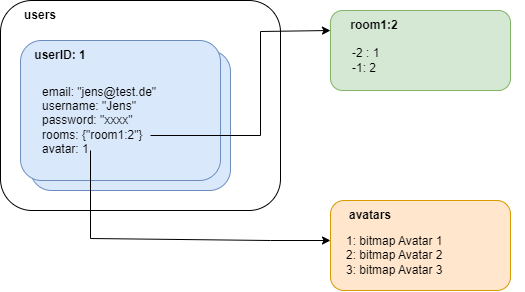
\includegraphics[width=0.7\textwidth]{datenmodellierung.png}
	\caption{Visualisierung des Datenmodells}
	\label{fig:datenmodell}
\end{figure}

In \autoref{fig:datenmodell} wird ein beispielhafter User \textit{Jens} betrachtet. Die Daten zu diesem User befinden sich im \textit{User}-Hash. Identifiziert wird der konkrete Hash, der \textit{Jens} repräsentiert, durch die ID \textit{1}. Jens hat einen Chatraum. Dieser ist zwischen ihm und dem User mit der ID \textit{2}. Wie bereits erwähnt ist jeder Raum ein eigenes \textit{Sorted-Set}, welches durch die zwei Teilnehmer identifiziert wird. Somit können mithilfe der Werte aus dem \textit{rooms} Feld \textit{Jens} Räume identifiziert und anschließend ausgelesen werden.

Jeder User hat das Feld \textit{avatar}, welches einen Integerwert enthält. Dieser Wert ist die Nummer des zugehörigen Avatars. \textit{Jens} hätte beispielsweise den Avatar mit dem Wert \textit{1}. Mithilfe dieser Information kann der korrekte Avatar in der Anwendung geladen und angezeigt werden.
\newpage
Bei der Verarbeitung gesendeter Nachrichten werden diese zum Einen mithilfe des \acs{Pub/Sub}-Prinzips und einem Websocket in Echtzeit im Frontend aktualisiert, zum Anderen werden diese im Backend in der \acs{Redis}-Datenbank ebenfalls persistent gespeichert (vgl. \autoref{subsec:pubsub}). 

\autoref{fig:ablauf} zeigt den beispielhaften Ablauf einer versendeten Nachricht. Es wird ersichtlich, dass die Nachricht auf zwei Wegen verarbeitet wird. Im linken Zweig wird die Nachricht serverseitig persistent in der \acs{Redis}-Datenbank gespeichert. Dies hat den Grund, dass die gesendete Nachricht auch zu einem späteren Zeitpunkt abrufbar sein soll. Im rechten Zweig wird die Nachricht mithilfe des \acs{Pub/Sub}-Prinzips und einem Websocket im Frontend in Echtzeit aktualisiert. Auf diese Weise kann der User die gesendete Nachricht sehen, ohne die Seite neu laden zu müssen.

\begin{figure}[h]
	\centering
	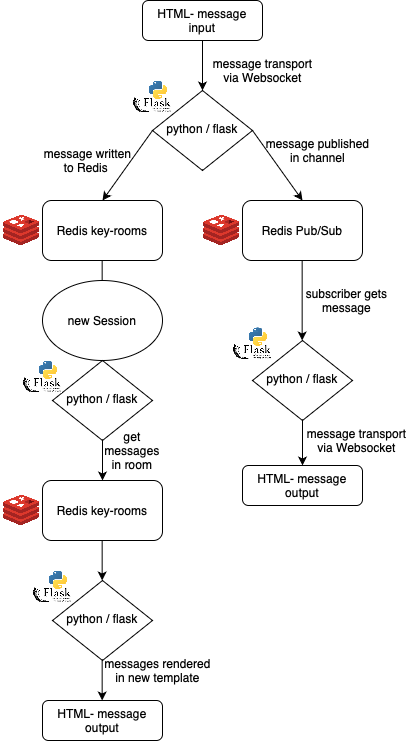
\includegraphics[width=0.5\textwidth]{ablauf.png}
	\caption{Beispielhafter Ablauf einer gesendeten Nachricht}
	\label{fig:ablauf}
\end{figure}

Dieser Ablauf wird bei jeder gesendet Nachricht ausgeführt, um es dem User zu ermöglichen die Daten in Echtzeit zu erhalten und diese persistent gespeichert zu haben.
